\chapter{Convergence of Random Variables}

\section{Modes of Convergence}

\subsection{Convergence in Mean}

\begin{definition}[Convergence in Mean]
	A sequence $\{X_n\}$ of real-valued random variables \textbf{converges in the r-th mean} ($r\geq1$) towards the random variable $X$, if
	\begin{enumerate}
		\item The r-th absolute moments $E(|X_n|^r)$ and $E(|X|^r)$ of $\{X_n\}$ and $X$ exist,
		\item $\lim_{n\to\infty}E\left(|X_n-X|^r\right)=0$.
	\end{enumerate}
	Convergence in the r-th mean is denoted by
	\begin{equation}
		X_n \stackrel{L^r}{\rightarrow} X.
	\end{equation}
\end{definition}

\subsection{Convergence in Probability}

\begin{definition}[Convergence in Probability]
	A sequence $\{X_n\}$ of real-valued random variables \textbf{converges in probability} towards the random variable $X$, if
	\begin{equation}
		\forall\varepsilon>0,\quad\lim_{n\to\infty}P\left(|X_n-X|>\varepsilon\right)=0.
	\end{equation}
	Convergence in probability is denoted by
	\begin{equation}
		X_n \stackrel{p}{\rightarrow} X.
	\end{equation}
\end{definition}

\subsection{Convergence in Distribution}

\begin{definition}[Convergence in Distribution] \label{def:convergence-in-distribution}
	A sequence $\{X_n\}$ of real-valued random variables is said to \textbf{converge in distribution}, or \textbf{converge weakly}, or \textbf{converge in law} to a random variable $X$, if
	\begin{equation}
		\lim_{n\to\infty}F_n(x)=F(x),
	\end{equation}
	for every number at $x\in\bbR$ which $F$ is continuous. Here $F_n$ and $F$ are the cumulative distribution functions of random variables $X_n$ and $X$, respectively.

	Convergence in distribution is denoted as
	\begin{equation}
		X_n \stackrel{d}{\rightarrow} X, \text{ or } X_n \Rightarrow X.
	\end{equation}
\end{definition}

\begin{itemize}
	\item Convergence in Distribution is the weakest form of convergence typically discussed since it is implied by all other types of convergence mentioned in this chapter.
	\item Convergence in Distribution does not imply that the sequence of corresponding probability density functions will also converge. However, according to Scheff's theorem, convergence of the probability density functions implies convergence in distribution.
\end{itemize}

\begin{theorem}[Portmanteau Lemma] \label{thm:portmanteau-lemma}
	$\{X_n\}$ converges in distribution to $X$, if and only if any of the following statements are true,
	\begin{itemize}
		\item $P(X_n\leq x)\rightarrow P(X\leq x)$, for all continuity points of the distribution of $X$.
		\item $Ef(X_n)\rightarrow Ef(X)$, for all bounded, continuous (Lipschitz) functions $f$.
		\item $\liminf_{n\rightarrow\infty}P\left(X_{n} \in G\right)\geq P\left(X_{\infty}\in G\right)$, for all open sets $G$.
		\item $\limsup_{n \rightarrow\infty}P\left(X_{n} \in K\right) \leq P\left(X_{\infty} \in K\right)$, for all closed sets $K$.
		\item $\lim_{n\rightarrow\infty}P\left(X_{n}\in A\right)=P\left(X_{\infty}\in A\right)$, for all Borel sets $A$ with $P\left(X_{\infty}\in \partial A\right)=0$.
	\end{itemize}
\end{theorem}

\begin{proof}

\end{proof}

\subsubsection{Continuous Mapping Theorem}

\begin{theorem}[Continuous Mapping Theorem] \label{thm:continuous-mapping-theorem}
	Let $g$ be a measurable function and $D_g=\{x:g \text{ is discontinuous at } x\}$ with $P(X\in D_g)=0$, then,
	\begin{equation}
		\begin{aligned}
			X_{n} \stackrel{d}{\rightarrow} X    & \Rightarrow g\left(X_{n}\right) \stackrel{\dif}{\rightarrow} g(X), \\
			X_{n} \stackrel{p}{\rightarrow} X    & \Rightarrow g\left(X_{n}\right) \stackrel{p}{\rightarrow} g(X),    \\
			X_{n} \stackrel{a.s.}{\rightarrow} X & \Rightarrow g\left(X_{n}\right) \stackrel{a.s.}{\rightarrow} g(X). \\
		\end{aligned}
	\end{equation}
	If in addition $g$ is bounded, then
	\begin{equation}
		Eg(X_n)\rightarrow Eg(X).
	\end{equation}
\end{theorem}

\begin{proof}

\end{proof}

\subsubsection{Slutsky's Theorem}

\begin{theorem}[Slutsky's Theorem] \label{thm:slutsky-theorem}
	Let $X_{n}, Y_{n}$ be sequences of random variables. If $X_{n}\stackrel{d}{\rightarrow}X$ and $Y_{n}\stackrel{p}{\rightarrow}c$, then
	\begin{enumerate}
		\item $X_{n}+Y_{n}\stackrel{d}{\rightarrow}X+c$.
		\item $X_{n}Y_{n}\stackrel{d}{\rightarrow}cX$.
		\item $X_{n}/Y_{n}\stackrel{d}{\rightarrow}X/c$, provided that $c$ is invertible.
	\end{enumerate}
\end{theorem}

\begin{proof}

\end{proof}

\begin{remark}
	However that convergence in distribution of $X_{n}\stackrel{d}{\rightarrow}X$ and $Y_{n}\stackrel{d}{\rightarrow}Y$ does in general not imply convergence in distribution of $X_n+Y_n\stackrel{d}{\rightarrow}X+Y$ or of $X_nY_n\stackrel{d}{\rightarrow}XY$.
\end{remark}

\subsubsection{The Delta Methods}

\begin{theorem}[Delta Method]
	Let $\{X_{n}\}$ be a sequence of random variables with
	\begin{equation}
		\sqrt{n}\left(X_{n}-\theta\right)\stackrel{d}{\rightarrow}N\left(0,\sigma^{2}\right)
	\end{equation}
	where $\theta$ and $\sigma$ are finite, then for any function $g$ with the property that $g^{\prime}(\theta)$ exists and is non-zero valued,
	\begin{equation}
		\sqrt{n}\left[g\left(X_{n}\right)-g(\theta)\right] \stackrel{d}{\rightarrow}N\left(0,\sigma^{2}\cdot\left[g^{\prime}(\theta)\right]^{2}\right)
	\end{equation}
\end{theorem}

\begin{proof}
	\begin{enumerate}
		\item  Under the assumption that $g^{\prime}(\theta)$ is continuous.

		      Since, $g^{\prime}(\theta)$ exists, with the first-order Taylor Approximation, that
		      \begin{equation*}
			      g(X_n)=g(\theta)+g^{\prime}(\tilde{\theta})(X_n-\theta)
		      \end{equation*}
		      where $\tilde{\theta}$ lies between $X_n$ and $\theta$.
		      Since $X_n\stackrel{p}{\rightarrow}\theta$, and $|\tilde{\theta}-\theta|<|X_n-\theta|$, then
		      \begin{equation*}
			      \tilde{\theta}\stackrel{p}{\rightarrow}\theta
		      \end{equation*}
		      Since $g^{\prime}(\theta)$ is continuous, by Continuous Mapping Theorem (\ref{thm:continuous-mapping-theorem}),
		      \begin{equation*}
			      g^{\prime}(\tilde{\theta})\stackrel{p}{\rightarrow}g^{\prime}(\theta)
		      \end{equation*}
		      and,
		      \begin{equation*}
			      \sqrt{n}\left(g(X_n)-g(\theta)\right)=\sqrt{n}g^{\prime}(\tilde{\theta})(X_n-\theta)
		      \end{equation*}
		      \begin{equation*}
			      \sqrt{n}\left(X_{n}-\theta\right)\stackrel{d}{\rightarrow}N\left(0,\sigma^{2}\right)
		      \end{equation*}
		      by Slutsky's Theorem (\ref{thm:slutsky-theorem}),
		      \begin{equation*}
			      \sqrt{n}\left[g\left(X_{n}\right)-g(\theta)\right] \stackrel{d}{\rightarrow}N\left(0,\sigma^{2}\cdot\left[g^{\prime}(\theta)\right]^{2}\right)
		      \end{equation*}
	\end{enumerate}
\end{proof}

\begin{theorem}[Second-order Delta Method]

\end{theorem}

\begin{remark}
	We can approximate the moments of a function $f(\cdot)$ of a random variable $X$ using Taylor expansions, provided that $f(\cdot)$ is sufficiently differentiable and that the moments of $X$ are finite. Suppose $\mu=\operatorname{E}\left(X\right)$, and $\sigma^{2}=\operatorname{Var}\left(X\right)$, with the Taylor expansions for the functions of random variables,
	\begin{equation}
		f\left(X\right)=f\left[\mu+\left(X-\mu\right)\right]\approx f\left(\mu\right)+f^{\prime}\left(\mu\right)\left(X-\mu\right)
	\end{equation}
	Thus,
	\begin{equation}
		\operatorname{E}\left[f\left(X\right)\right]\approx\operatorname{E}\left[f\left(\mu\right)\right],\quad\operatorname{Var}\left[f(X)\right]\approx\left[f^{\prime}\left(\mu\right)\right]^{2}\cdot\sigma^{2}
	\end{equation}
\end{remark}

\subsubsection{L\`evy' s Continuity Theorem}

\begin{theorem}[L\`evy' s Continuity Theorem]
	Let $\mu_{n},1\leq n\leq\infty$ be probability measures with ch. f. $\varphi_{n}$.
	\begin{enumerate}
		\item If $\mu_{n}\stackrel{d}{\rightarrow}\mu_{\infty}$, then $\varphi_{n}(t)\rightarrow\varphi_{\infty}(t)$ for all $t$.
		\item If $\varphi_{n}(t)$ converges pointwise to a limit $\varphi(t)$ that is continuous at $0$, then the associated sequence of distributions $\mu_{n}$ is tight and converges weakly to the measure $\mu$ with characteristic function $\varphi$.
	\end{enumerate}
\end{theorem}

\begin{proof}

\end{proof}

\subsubsection{Cram\'er-Wold Theorem}

\begin{theorem}[Cram\'er-Wold Theorem] \label{thm:cramer-wold-theorem}

\end{theorem}

\subsection{Almost Sure Convergence}

\begin{definition}[Almost Sure Convergence]
	A sequence $\{X_n\}$ of real-valued random variables converges \textbf{almost sure} or \textbf{almost everywhere} or \textbf{with probability 1} or \textbf{strongly} towards the random variable $X$, if
	\begin{equation}
		P\left(\lim_{n\to\infty}X_n=X\right)=1.
	\end{equation}
	Almost sure convergence is denoted by
	\begin{equation}
		X_n \stackrel{a.s.}{\rightarrow} X.
	\end{equation}
\end{definition}

\begin{remark}

\end{remark}

\subsection{Convergence in Uninform}

\begin{definition}[Convergence in Uninform]

\end{definition}

\subsection{Asymptotic Notation}

\begin{definition}
	A sequence $\{A_n\}$ of real-valued random variables is of smaller order in probability than a sequence $\{B_n\}$, if
	\begin{equation}
		\frac{A_n}{B_n}\stackrel{p}{\rightarrow}0.
	\end{equation}
	Smaller order in probability is denoted by
	\begin{equation}
		A_n=o_p(B_n).
	\end{equation}
	Particularly,
	\begin{equation}
		A_n=o_p(1)\iff A_n\stackrel{p}{\rightarrow}0.
	\end{equation}
\end{definition}

\begin{definition}
	A sequence $\{A_n\}$ of real-valued random variables is of smaller order than or equal to a sequence $\{B_n\}$ in probability, if
	\begin{equation}
		\forall\varepsilon>0\;\exists M_\varepsilon,\quad\lim_{n\rightarrow\infty} P\left(|A_n|\leq M_\varepsilon|B_n|\right)\geq 1-\varepsilon.
	\end{equation}
	Smaller order than or equal to in probability is denoted by
	\begin{equation}
		A_n=O_p(B_n).
	\end{equation}
\end{definition}

\begin{definition}
	A sequence $\{A_n\}$ of real-valued random variables is of the same order as a sequence $\{B_n\}$ in probability, if
	\begin{equation}
		\forall\varepsilon>0\;\exists m_{\varepsilon}<M_{\varepsilon},\quad\lim_{n\rightarrow\infty} P\left(m_{\varepsilon}<\frac{|A_{n}|}{|B_{n}|}<M_{\varepsilon}\right)\geq 1-\varepsilon.
	\end{equation}
	The same order in probability is denoted by
	\begin{equation}
		A_{n}\asymp_{p}B_{n}.
	\end{equation}
\end{definition}

\section{Relationships of Modes}

\begin{lemma}
	If $p>0$ and $E\left|Z_{n}\right|^{p}\rightarrow 0$, then
	\begin{equation}
		Z_{n}\stackrel{p}{\rightarrow}0.
	\end{equation}
\end{lemma}

\begin{proof}

\end{proof}

\begin{theorem}
	If $X_{n}\stackrel{p}{\rightarrow}X$, then
	\begin{equation}
		X_{n}\stackrel{d}{\rightarrow}X,
	\end{equation}
	and that, conversely, if $X_{n}\stackrel{d}{\rightarrow}c$, where $c$ is a constant, then
	\begin{equation}
		X_{n}\stackrel{p}{\rightarrow}c.
	\end{equation}
\end{theorem}

\begin{proof}
	\begin{enumerate}
		\item $\forall\varepsilon>0$, at fixed point $x$, since if $X_n\leq x$ and $|X_n-X|\leq\varepsilon$, then $X\leq x+\varepsilon$, then
		      \begin{equation*}
			      \{X\leq x+\varepsilon\}\subset\{X_n\leq x\}\cup\{|X_n-X|>\varepsilon\},
		      \end{equation*}
		      similarly, if $X\leq x-\varepsilon$ and $|X_n-X|\leq\varepsilon$, then $X_n\leq x$, then
		      \begin{equation*}
			      \{X_n\leq x\}\subset\{X\leq x-\varepsilon\}\cup\{|X_n-X|>\varepsilon\},
		      \end{equation*}
		      then, by the union bound,
		      \begin{equation*}
			      \begin{gathered}
				      P\left(X\leq x+\varepsilon\right)\leq P\left(X_n\leq x\right)+P\left(|X_n-X|>\varepsilon\right),\\
				      P\left(X_n\leq x\right)\leq P\left(X\leq x-\varepsilon\right)+P\left(|X_n-X|>\varepsilon\right).\\
			      \end{gathered}
		      \end{equation*}
		      So, we got
		      \begin{equation*}
			      \begin{gathered}
				      P\left(X\leq x+\varepsilon\right)-P\left(|X_n-X|>\varepsilon\right)\leq P\left(X_n\leq x\right) \\
				      \leq P\left(X\leq x-\varepsilon\right)+P\left(|X_n-X|>\varepsilon\right)
			      \end{gathered}
		      \end{equation*}
		      As $n\rightarrow\infty$, $P\left(|X_n-X|>\varepsilon\right)\rightarrow 0$, then
		      \begin{equation*}
			      \begin{gathered}
				      P\left(X\leq x-\varepsilon\right)\leq\lim_{n\rightarrow\infty}P\left(X_n\leq x\right)\leq P\left(X\leq x+\varepsilon\right) \\
				      \Rightarrow F(x-\varepsilon)\leq \lim_{n\rightarrow\infty}F_n(x)\leq F(x+\varepsilon)
			      \end{gathered}.
		      \end{equation*}
		      By the property of distribution (Theorem \ref{thm:distribution-function-property}), as $\varepsilon\rightarrow 0$, then
		      \begin{equation*}
			      \lim_{n\rightarrow\infty}F_n(x)=F(x),
		      \end{equation*}
		      which means,
		      \begin{equation*}
			      X_n\stackrel{d}{\rightarrow}X.
		      \end{equation*}
		\item
		      Since $X_{n}\stackrel{d}{\rightarrow}c$, where $c$ is a constant, then $\forall\varepsilon>0$,
		      \begin{equation*}
			      \begin{gathered}
				      \lim_{n\rightarrow\infty}P(X_n\leq c+\varepsilon)=1\Rightarrow\lim_{n\rightarrow\infty}P(X_n>c+\varepsilon)=0\\
				      \lim_{n\rightarrow\infty}P(X_n\leq c-\varepsilon)=0.\\
			      \end{gathered}
		      \end{equation*}
		      Therefore,
		      \begin{equation*}
			      P\left(\left|X_n-c\right|<\varepsilon\right)=0,
		      \end{equation*}
		      which means
		      \begin{equation*}
			      X_n\stackrel{p}{\rightarrow}c.
		      \end{equation*}
	\end{enumerate}
\end{proof}

\begin{theorem}
	If $X_{n}\stackrel{a.s.}{\rightarrow}X$, then
	\begin{equation}
		X_{n}\stackrel{p}{\rightarrow}X.
	\end{equation}
\end{theorem}

\begin{proof}

\end{proof}

\begin{theorem}
	$X_n\stackrel{p}{\rightarrow}X$ if and only if for all subsequence $X_{n(m)}$ exists a further subsequence $X_{n(m_k)}$, such that
	\begin{equation}
		X_{n(m_k)}\stackrel{a.s.}{\rightarrow}X.
	\end{equation}
\end{theorem}

\begin{lemma} \label{lem:distribution-to-probability}
	If $F_n\stackrel{d}{\rightarrow}F_\infty$, then there are random variables $Y_n,1\leq n\leq \infty$, with distribution $F_n$ so that
	\begin{equation}
		Y_n\stackrel{a.s.}{\rightarrow}Y_\infty.
	\end{equation}
\end{lemma}

\begin{figure}[htp]
	\centering
	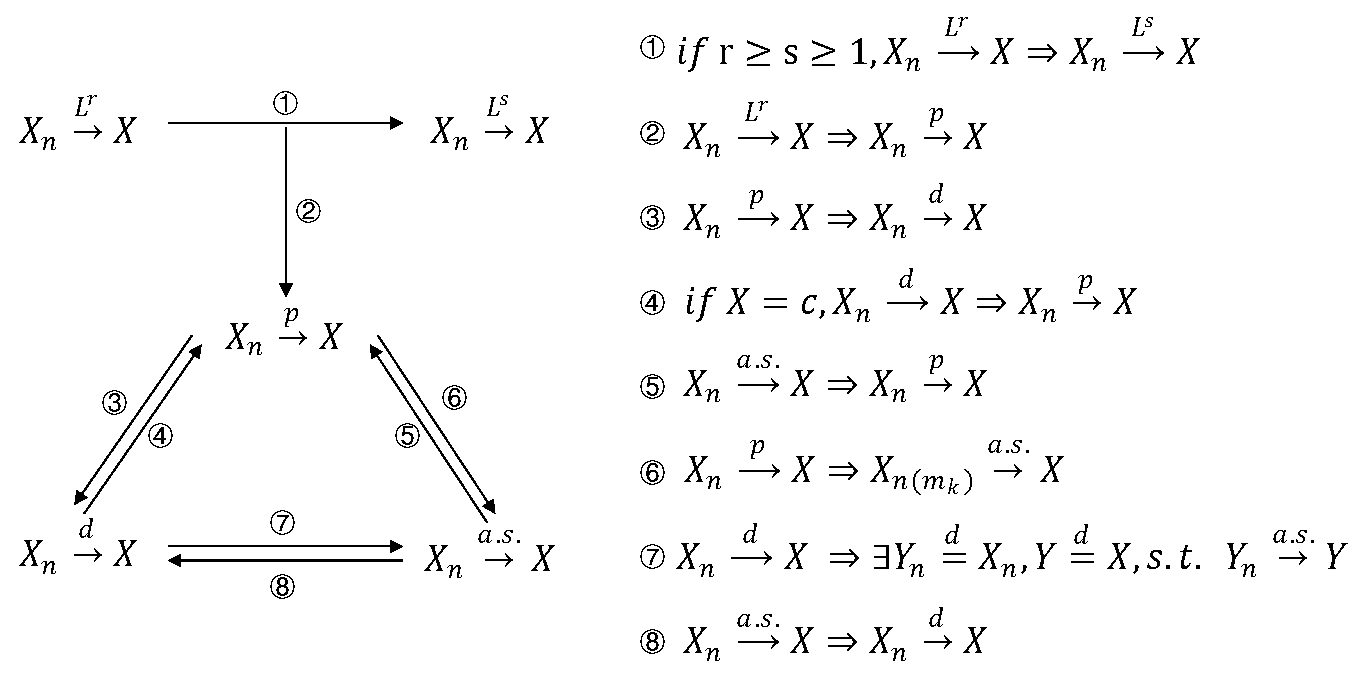
\includegraphics[width=0.9\textwidth]{./probability-theory/figures/relation-of-convergences.eps}
	\caption{Relations of Convergence of Random Variables}
\end{figure}

% % \paragraph*{Limits of Sequences of Distributions $\{F_n\}$}

% \begin{theorem}[Helly's Selection Theorem]
%     For every sequence $F_{n}$ of distribution functions, there is a subsequence $F_{n}(k)$ and a right continuous nondecreasing function $F$ so that $\lim_{k\rightarrow\infty}F_{n(k)}(y)=F(y)$ at all continuity points $y$ of $F$.
% \end{theorem}

% \begin{theorem}
%     Every subsequential limit is the distribution function of a probability measure if and only if the sequence $F_{n}$ is tight, i.e., for all $\epsilon>0$ there is an $M_{\epsilon}$ so that
%     \begin{equation}
%         \limsup_{n\rightarrow\infty}1-F_{n}\left(M_{\epsilon}\right)+F_{n}\left(-M_{\epsilon}\right)\leq\epsilon.
%     \end{equation}
% \end{theorem}
